\paragraph{}Este ap�ndice apresenta a ferramenta WaveInspector, criada pelo autor para facilitar a inspe��o manual de ondas, a fim de comparar os valores medidos manualmente com os resultados do algoritmo apresentado no projeto.

\begin{figure}[h]
	\centering
	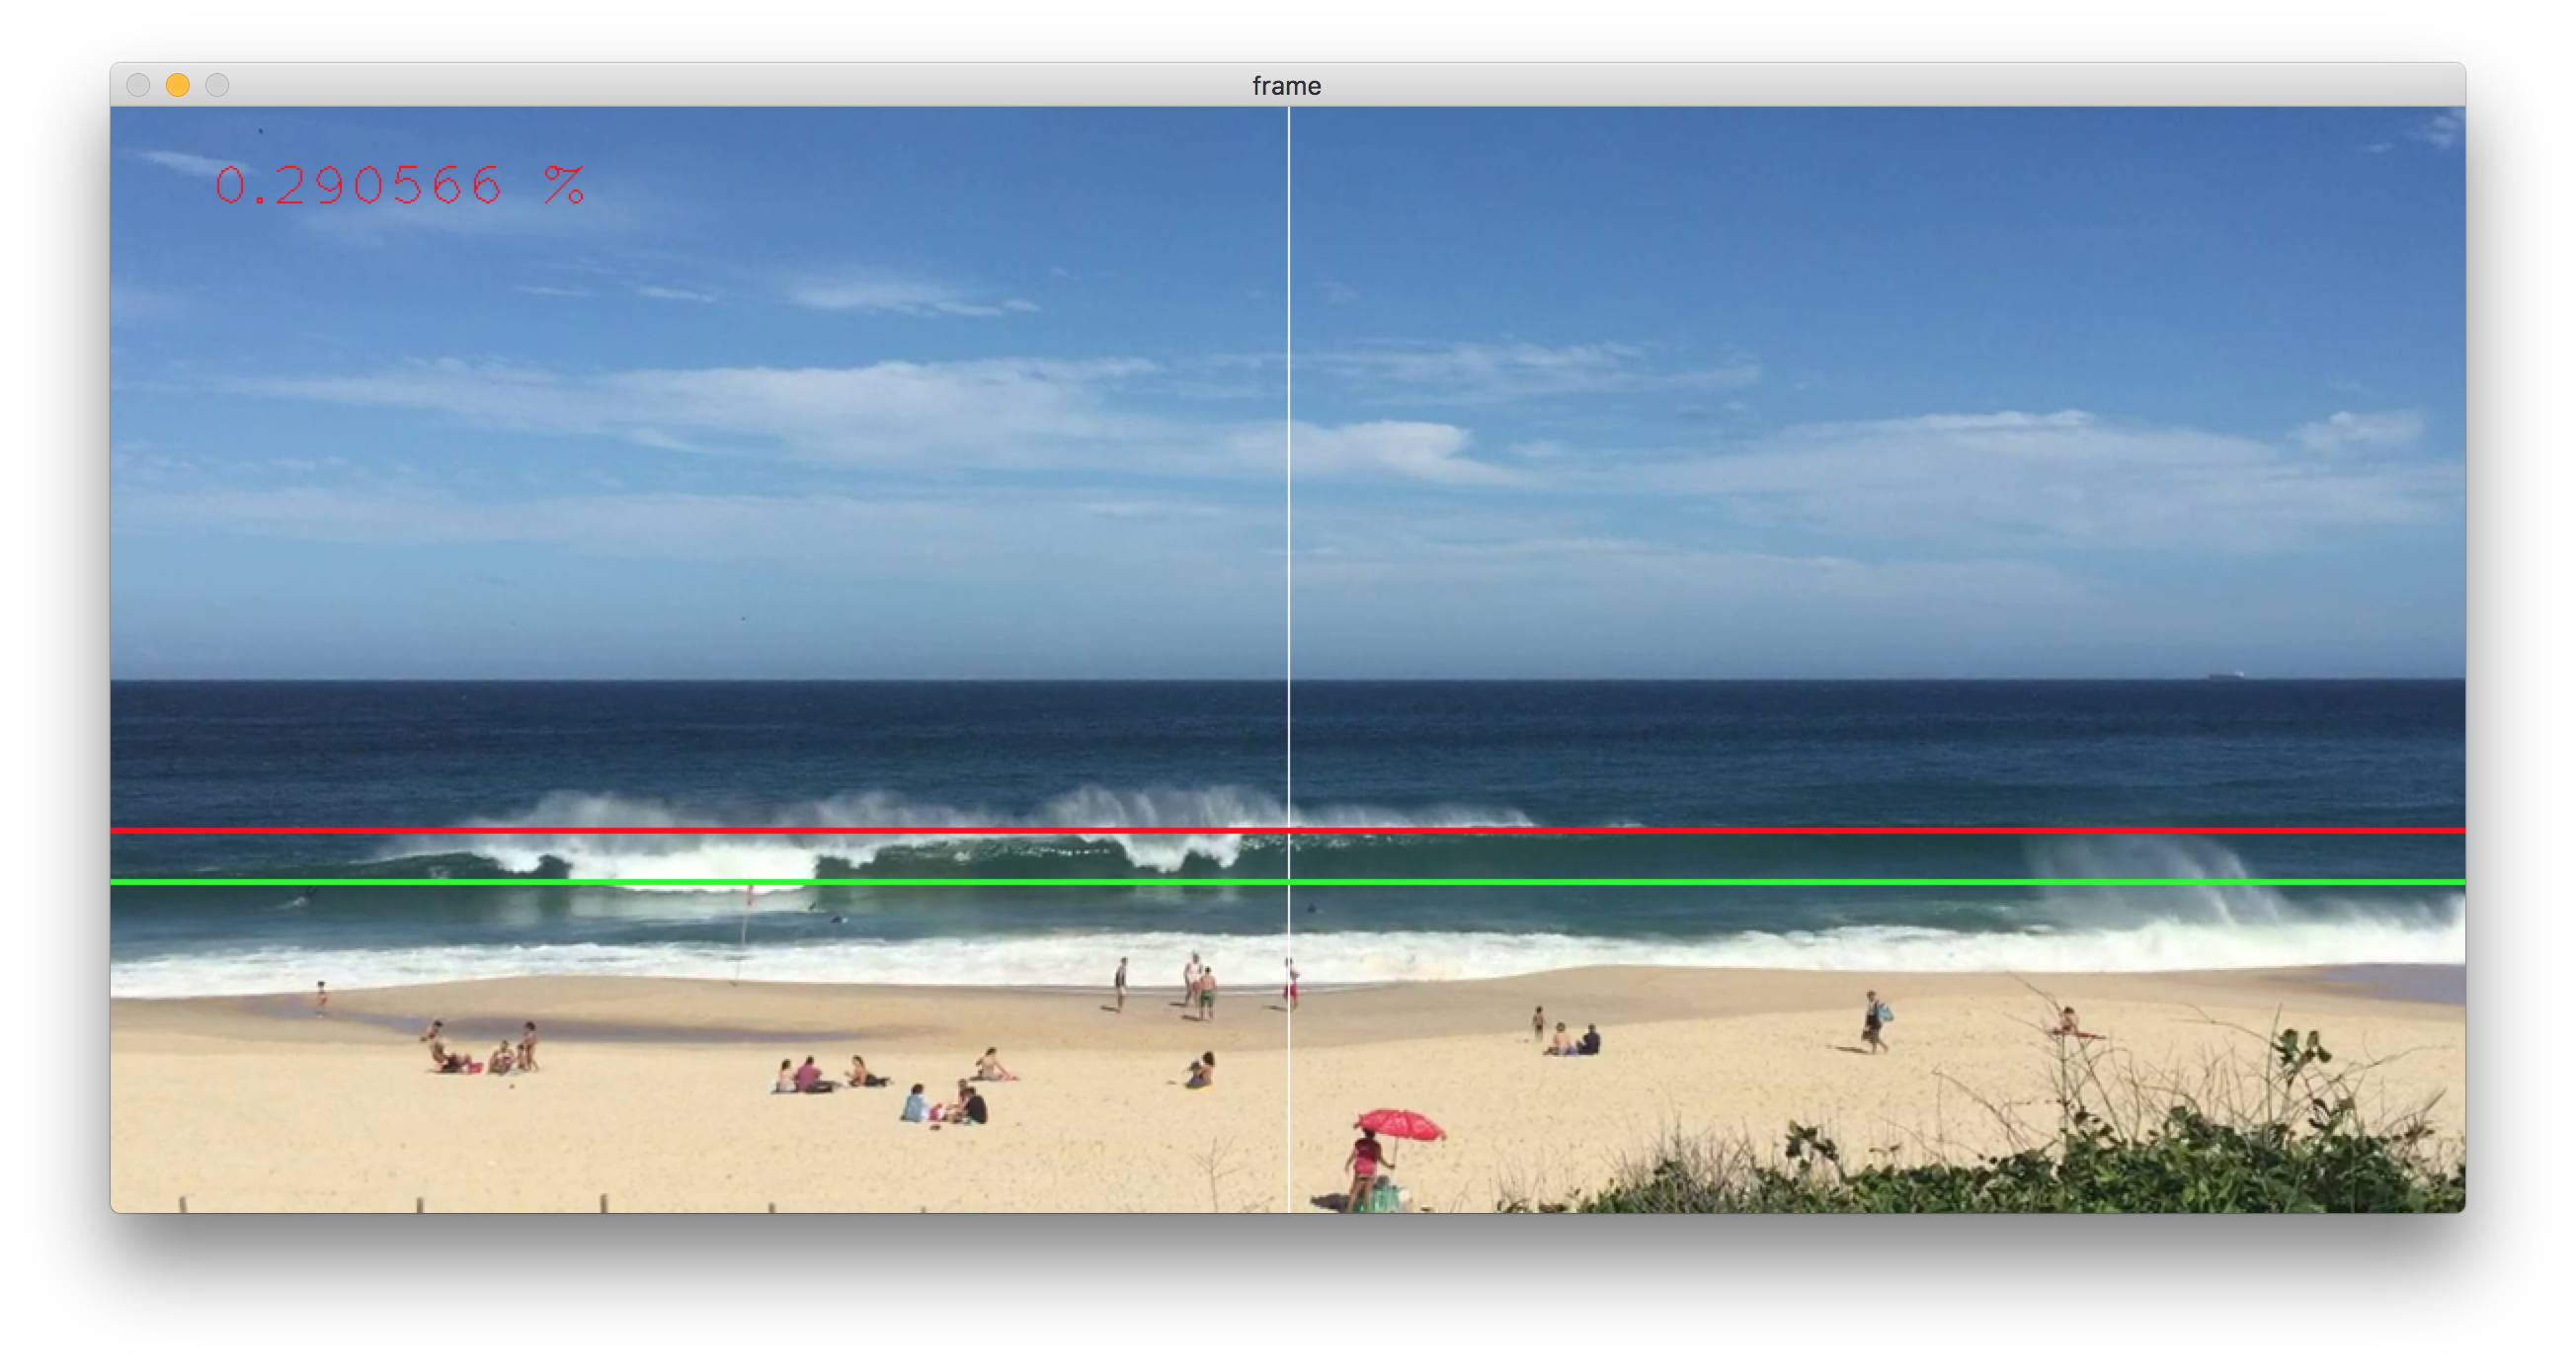
\includegraphics[width=\textwidth,keepaspectratio]{screenshot-waveinspector.png}
	\caption[\small{Ferramenta WaveInspector com uma onda detectada pelo usu�rio.}]{\small{Ferramenta WaveInspector com uma onda detectada pelo usu�rio.}}
	\label{FigWaveInspector}
\end{figure}

\paragraph{}O funcionamento da ferramenta � simples: ao inici�-la uma janela com o v�deo em andamento � exibida, contendo a porcentagem do v�deo que j� foi exibida e uma linha vertical indicando o centro da imagem. O inspetor pode interagir com o v�deo utilizando o teclado e o mouse. As teclas "p" e "c" s�o utilizadas para pausar e continuar a execu��o do v�deo. Uma vez pausado, o mouse pode ser utilizado para marcar o ponto m�ximo e o ponto m�nimo de uma onda. O ponto m�ximo � representado por uma linha horizontal vermelha, enquanto o ponto m�nimo � representado por uma linha verde. Os cliques sucessivos alteram o controle de cada ponto -- o primeiro clique posiciona o ponto m�ximo, o segundo clique o ponto m�nimo, o terceiro o ponto m�ximo novamente e assim por diante. Ap�s selecionar os pontos desejados, a tecla "s" adiciona a onda marcada em uma lista. Para descartar a onda marcada basta pressionar a tecla "c" para retomar a execu��o do v�deo. Por �ltimo, tamb�m com o v�deo pausado, as teclas "f" e "b" podem ser utilizadas para adiantar ou atrasar o v�deo. No final da execu��o do v�deo, os dados ser�o salvos em um arquivo "waves.txt". Os \textit{frames} contendo as ondas identificadas ser�o salvos em um diret�rio "output\_waves/wave\_inspector/".

\paragraph{}O c�digo da ferramenta WaveInspector est� ilustrado abaixo:

\lstinputlisting[tabsize=2]{../src/waveInspector.cpp}